% Section content template for individual Educative lessons
% This file contains the actual content for a specific section
% Generated from Educative API section content

% Section: High-Level Design of Sharded Counters
% Section ID: 6126387596886016
% Section Slug: high-level-design-of-sharded-counters
% Generated: 2025-12-07T22:16:25.575570

\subsection{High-level solution sketch}\label{iYlUmgHvgddn-QGLfcIIW}
\\
Managing millions of tweet likes requires many counters operating on many nodes. To manage these counters, we need an efficient system that can provide high performance and scalability as the number of users grows.
\\
What will happen when a single tweet on Twitter gets a million likes, and the application server receives a write request against each like to increment the relevant counter? These millions of requests are eventually serialized in a queue for data consistency. Such serialization is one way to deal with concurrent activity, though at the expense of added delay. Real -time applications want to keep the quality of experience high by providing as minimum as possible latency for the end user.
\\
Let's see the illustration below to understand this problem:

\begin{figure}[htbp]
 \centering
 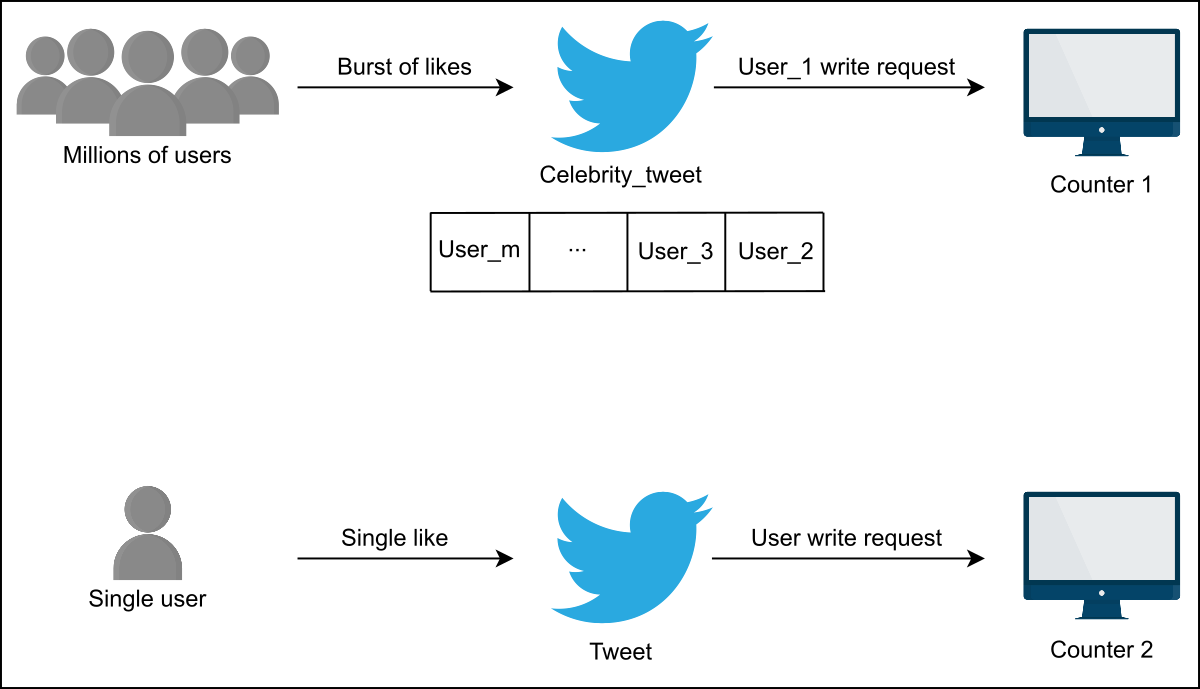
\includegraphics[width=0.5\textwidth]{Images/chapter_24/section_6126387596886016/4647427739222016.png}
 \caption{Celebrity vs. common people tweet}
\end{figure}

A single counter for each tweet posted by a celebrity is not enough to handle millions of users. The solution to this problem is a \textbf{sharded counter}, also known as a distributed counter, where each counter has a specified number of shards as needed. These shards run on different computational units in parallel. We can improve performance and reduce contention by balancing the millions of write requests across shards.
\\
First, a write request is forwarded to the specified tweet counter when the user likes that tweet. Then , the system chooses an available shard of the specified tweet counter to increment the like count. Let
's look at the illustration below to understand sharded counters having specified shards:

\begin{figure}[htbp]
 \centering
 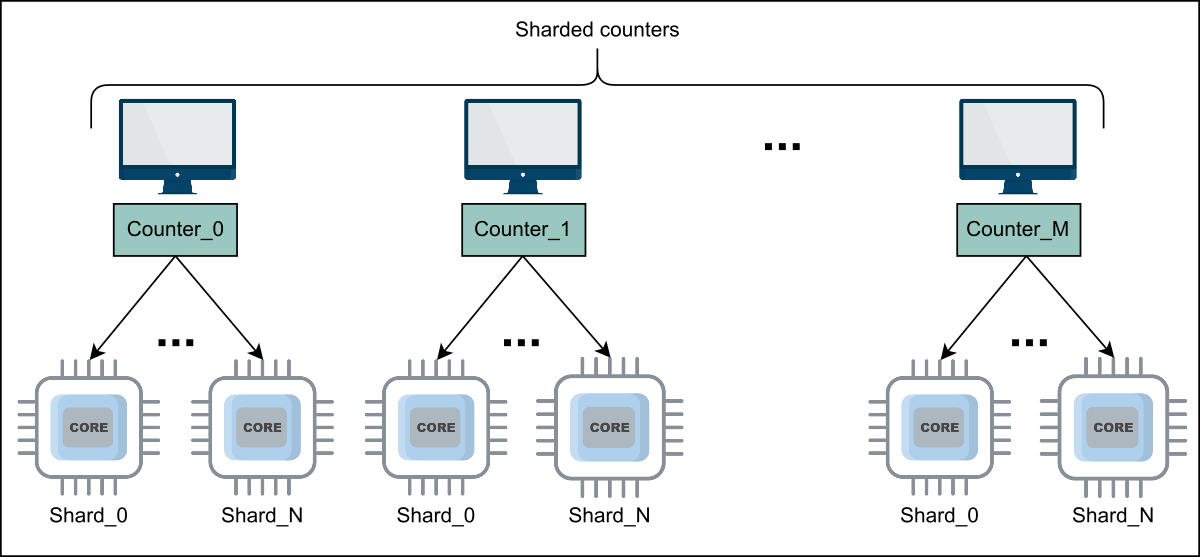
\includegraphics[width=0.5\textwidth]{Images/chapter_24/section_6126387596886016/6509805661585408.png}
 \caption{Counters and their shards working on different computational units}
\end{figure}

In the above illustration, the total number of shards per counter is \protect\phantomsection\label{katex_inline_5FcE4g17BDG7nUn8nSbmZ}{{{\(\text{(N+1)}\)}}}. We 'll use an appropriate value for \protect\phantomsection\label{katex_inline_NF3jBwBV4gqApNmSyJY67}{{{\(\text{N}\)}}} according to our needs. Let
's discuss an example to understand how sharded counters handle millions of write and read requests for a single post.
\\
Let's assume that a famous YouTube channel with millions of subscribers uploads a new video. The server receives a burst of write requests for video views from worldwide users. First , a new counter initiates for a newly uploaded video. The server forwards the request to the corresponding counter, and our system chooses the shard randomly and updates the shard value, which is initially zero. In contrast, when the server receives read requests, it adds the values of all the shards of a counter to get the current total.
\\
We can use a sharded counter for every scenario where we need scalable counting (such as Facebook posts and YouTube videos).

\subsection{API design for sharded counters}\label{hQBMYAzE2Uyc2Y3RJhGhK}
\\
This section discusses the APIs that will be called for sharded counters. Our API design will help us understand the interactions between sharded counters and their callers. To make our discussion concrete, we'll discuss each API function in the context of Twitter. Let
's develop APIs for each of the following functionalities:

\begin{itemize}
\item
\protect\phantomsection\label{EUPuA7wanl7FBom9zp1iS}
Create counter
\item
\protect\phantomsection\label{-WN6CCiCs3z0dnG7C2Dla}
Write counter
\item
\protect\phantomsection\label{Q1HirhUwi3iXfadOggQgN}
Read counter
\end{itemize}
\\
Although the above list of API functions is not exhaustive, they represent some of the most important ones.

\subsubsection{Create counter}\label{jaPHT5qkpAAcA5yq7WS4u}
\\
The \textbackslash{createCounter} API initializes a distributed counter for use. The \textbackslash{createCounter} API is given below:

\begin{lstlisting}[language=JavaScript]
createCounter(counter_id, number_of_shards)
\end{lstlisting}

\begin{table}[htbp]
\centering
\small
\adjustbox{max width=\textwidth}{
\begin{tabular}{|p{0.210\textwidth}|p{0.740\textwidth}|}
\hline
\textbf{Parameter} & \textbf{Description} \\
\hline
\hline
\texttt{counter\_id} & It represents the unique ID of the counter. The caller of this API can use a sequencer to get a unique identifier. See the lesson on sequencer building blocks for more details. \\
\hline
\texttt{number\_of\_shards} & It specifies the number of shards for the counter. \\
\hline
\end{tabular}
}
\end{table}

We can use an appropriate data store to keep our metadata, which includes counter identifiers, their number of shards, and the mapping of shards to physical machines.
\\
Let's consider Twitter as an example to understand how an application uses the above API. The
\textbackslash{createCounter} API is used when a user posts something on social media. For instance, if a user posts a tweet on Twitter, the application server calls the \textbackslash{createCounter} API. The content\_type parameter is the post type that the system uses to decide the number of counters that need to be created. For example, the system needs a view counter only if the tweet contains a video clip.
\\
To find an appropriate value for number\_of\_shards, we can use the following heuristics:

\begin{itemize}
\item
\protect\phantomsection\label{LkAgv8aPFupeMZKmUowAl}
The followers\_count parameter denotes the followers' count of the user who posts a tweet.
\item
\protect\phantomsection\label{oJfYtiAjBleQGG5Bge36H}
The post\_type parameter specifies whether the post is public or protected. Protected tweets are for the followers only, and in this case, we have a better predictor of the number of shards.
\end{itemize}

\subsubsection{Write counter}\label{rjM9sXsz0k41SzVMSAHN_}
\\
The \textbackslash{writeCounter} API is used when we want to increment (or decrement) a counter. In reality, a specific shard of the counter is incremented or decremented, and our service makes that decision based on multiple factors, which we'll discuss later. The
\textbackslash{writeCounter} API is given below:

\begin{lstlisting}[language=JavaScript]
writeCounter(counter_id, action_type)
\end{lstlisting}

\begin{table}[htbp]
\centering
\small
\adjustbox{max width=\textwidth}{
\begin{tabular}{|p{0.210\textwidth}|p{0.740\textwidth}|}
\hline
\textbf{Parameter} & \textbf{Description} \\
\hline
\hline
\texttt{counter\_id} & It is the unique identifier (provided at the time of counter creation). \\
\hline
\texttt{action\_type} & It specifies the intended action (increment or decrement value of the counter). We extract the required information about the counter from our data store. \\
\hline
\end{tabular}
}
\end{table}

In our Twitter example, the \textbackslash{writeCounter} API is used when users act (by liking, replying, and so on) on someone else's post or their own post.

\subsubsection{Read counter}\label{85Wx1-Eyn1KxXuHFzJx7M}
\\
The \textbackslash{readCounter} API is used when we want to know the current value of the counter. Our system fetches appropriate information from the datastore to collect value from all shards. The
\textbackslash{readCounter} API is given below:

\begin{lstlisting}[language=JavaScript]
readCounter(counter_id)
\end{lstlisting}

\begin{table}[htbp]
\centering
\small
\adjustbox{max width=\textwidth}{
\begin{tabular}{|p{0.210\textwidth}|p{0.740\textwidth}|}
\hline
\textbf{Parameter} & \textbf{Description} \\
\hline
\hline
\texttt{counter\_id} & It is the unique identifier (provided at the time of counter creation). \hfill\break For Twitter, the \texttt{counter\_id} will be decided based on the following metrics: \hfill\break The \texttt{tweet\_id} specifies the tweet\textquotesingle s unique ID for which the request is generated. We can use \texttt{tweet\_id} to get the \texttt{counter\_id} for all the counters of the features (likes, retweets, and so on). \\
\hline
\end{tabular}
}
\end{table}

The \textbackslash{readCounter} API is called when users want to see the number of likes or view counts on a specific tweet. Usually , this API is triggered by another API when users want to see their home or user timeline.
\\
The following section will discuss what happens in the back-end system when all the above APIs are called.

% End of section content